\documentclass[a4paper]{scrbook}

\usepackage[utf8]{inputenc}
\usepackage{graphicx}
\usepackage{booktabs}
\usepackage{url}
\usepackage{relsize}
\usepackage{hyperref}
\usepackage{libertine}
\usepackage{ifthen}
\usepackage{fancyhdr}

%%%%%%%%%%%%%%%%%%%%%%%%%%%%%%%%%%%%%%%%%%%%%%%%%%%%%%%%%%%%%%%%%%%%%%%%%%%%%%%%
% Replace these values
%%%%%%%%%%%%%%%%%%%%%%%%%%%%%%%%%%%%%%%%%%%%%%%%%%%%%%%%%%%%%%%%%%%%%%%%%%%%%%%%
\newcommand{\thesistitleDE}{Deutscher Titel\\Maximal zwei Zeilen}
\newcommand{\thesistitleEN}{English Title\\Two lines at most}
\newcommand{\student}{Firstname Lastname}
\newcommand{\matrnr}{123456}
\newcommand{\submissiondate}{XX.\ Monat 20XX}
\newcommand{\supervisor}{Prof.~Dr.~Rehrnert}
\newcommand{\secsupervisor}{Prof.~Dr.~Zweitprüfer} % Unset this variable if no second supervisor is required
\newcommand{\faculty}{Angewandte Informatik}

% Select your course of studies here
%\newcommand{\studies}{Bachelor Cybersecurity}
%\newcommand{\studies}{Bachelor Künstliche Intelligenz}
\newcommand{\studies}{Bachelor Angewandte Informatik}
%\newcommand{\studies}{Master Angewandte Informatik}
%\newcommand{\studies}{Bachelor Elektro- und Informationstechnik}
%\newcommand{\studies}{Master Elektro- und Informationstechnik}
%\newcommand{\studies}{Bachelor Medientechnik}
%\newcommand{\studies}{Master Medientechnik}
%\newcommand{\studies}{Master of Applied Research}

% Select the targeted degree here
\newcommand{\degree}{Bachelor of Engineering (B.Eng.)}
%\newcommand{\degree}{Master of Engineering (M.Eng.)}
%\newcommand{\degree}{Master of Science (M.Sc.)}
%%%%%%%%%%%%%%%%%%%%%%%%%%%%%%%%%%%%%%%%%%%%%%%%%%%%%%%%%%%%%%%%%%%%%%%%%%%%%%%%

\renewcommand*{\UrlFont}{\ttfamily\smaller\relax}

\begin{document}
\pagestyle{headings}
\pagenumbering{roman}
\setkomafont{title}{\huge \scshape}
\begin{titlepage}
\begin{center}
	{\usekomafont{subject}
	Technische Hochschule Deggendorf\\
	Fakultät \faculty\par}
	\vspace{.2cm}
{\Large Studiengang \studies\\}
\vspace{6\baselineskip}
{\Huge\usekomafont{title}\thesistitleDE\par}
\vspace{1cm}
{\Huge\usekomafont{title}\thesistitleEN\par}
\vspace{6\baselineskip}

\usekomafont{publishers}
Masterarbeit zur Erlangung des akademischen Grades:

	\vspace{.2cm}
	\emph{\degree}
	\vspace{.2cm}

an der Technischen Hochschule Deggendorf\\
\end{center}
\vfill
\parbox[t]{.4\textwidth}{\usekomafont{author}
	Vorgelegt von:\\
	\student\\
	Matrikelnummer: \matrnr\par
	\vspace{\baselineskip}
	Am: \submissiondate\par
}
\hfill
\parbox[t]{.4\textwidth}{\usekomafont{author}
Prüfer:\\
\supervisor%
}
\end{titlepage}
\cleardoublepage\par


\chapter*{Abstract}
\addcontentsline{toc}{chapter}{Abstract}
The abstract goes here

\tableofcontents

\cleardoublepage%
\setcounter{page}{1}
\pagenumbering{arabic}
\chapter{The first chapter}
Remember that every element---chapter, section, or subsection---should start with text.
It is bad style to have one headline immediately followed by another headline. Instead,
use the space to describe what comes next.

\section{My first section}
The text of the thesis should be structured in chapters, sections,
and subsections. It may be a good idea to contain each chapter
in its own file.

\section{Some hints on layout}
Here are some hints on how to layout and structure the thesis document.

\subsection{On sections and introductory texts}
Remember that it is bad style to have only a single element on any level.
A section either contains at least two subsections or none at all. If you
are tempted to introduce a lone subsection, stop and rethink your structure.

\subsection{Lists}
Lists can be created with the
\begin{itemize}
	\item itemize
	\item environment
\end{itemize}
or the
\begin{enumerate}
	\item enumerate
	\item environment
\end{enumerate}
\subsection{Graphics}
Pictures can be included using includegraphics. They are automatically placed
by the typesetting engine. All figures have to be described in the text, where
they can be referenced by their label like this: Fig.~\ref{fig:myfig}. If there
are a lot of figures, it may be a good idea to create a separate folder for them.
If the automatic placement of figures produces bad results, add a placement
specifier.

\begin{figure}
	\centering
	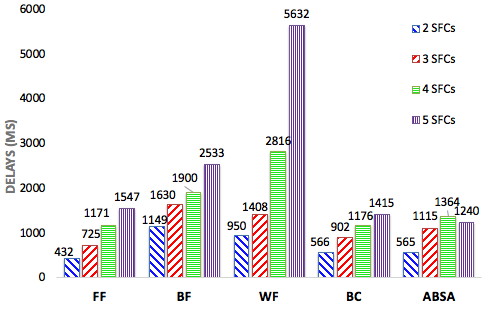
\includegraphics[width=.8\linewidth]{DelayComp.png}
	\caption{All figures require a caption, describing the content}\label{fig:myfig}
\end{figure}

\subsection{Tables}

Tables are best set using the booktabs package. They work by using the
table and tabular environments enclosed in each other.
Like figures, tables are floating elements that are automatically placed
by the typesetting engine. They can and should be referenced in a similar
way: Table~\ref{tab:mytable}. Tables only have horizontal lines---do not
attempt to introduce vertical lines.

\begin{table}[b]
	\centering % Use \centering to align to center
\begin{tabular}{lcr} % [l]eft, [c]enter, [r]ight
	\toprule
	First column header & Centered text & Right aligned \\
	\midrule
	Left aligned	& Centered &	7.0 \\
	A second row	& Some text &	38.5 \\
	\bottomrule
\end{tabular}
\caption{A floating table}%
\label{tab:mytable}
\end{table}

\subsection{Bibliography}

The bibliography is managed with BibTeX. Add entries to the \verb'reference.bib'
file in the main directory. You can reference them with the cite command~\cite{someref}.
BibTeX info for scientific publications is found in the common literature repositories
(Springer, Elsevier, IEEE). A program like JabRef might be useful for managing the
literature database.


\chapter{More info}

More information on LateX can be found online. There is a wikibook on LaTeX
to be found here: \url{https://en.wikibooks.org/wiki/LaTeX}. Also, the
TeX section of stackexchange.com provides answers to almost any question:
\url{https://tex.stackexchange.com/}~\cite{stackexchange}.


\bibliographystyle{IEEEtran}
\bibliography{references}
\end{document}
